\section{Context Overview}
\label{res-sec:context-overview}

This section presents data sources concerning the document survey mainly. Section \ref{results-ss:general-overview} covers sources related to a general perspective and Section \ref{results-ss:classroom-data} encompasses from \gls{MIS} class data.

\subsection{General Perspective}
\label{results-ss:general-overview}

I divided the general perspective into two kinds of data sources: curricula and \acrfull{UFPE} open data (see Table \ref{tbl:general-data-sources})\footnote{All these documents are available on this \gls{Ph.D.} public repository: \url{https://github.com/bispojr/phd-info}.}.

\begin{table}[htb]
\caption{List of data sources from the general perspective (curricula and \acrshort{UFPE} open data).}
\label{tbl:general-data-sources}
\centering
\rowcolors{1}{}{lightgray}
\begin{tabular}{
    >{\centering\arraybackslash}m{3cm}|
    >{\centering\arraybackslash}m{11cm}
}
    \hline
    \textbf{Abbreviation} &
    \textbf{Description} \\
    
    \hline
    \acrshort{DS-IC}1 &
    \acrfull{CC2020} \\

    \acrshort{DS-IC}2&
    \acrfull{IS2020} \\

    \acrshort{DS-IC}3 &
    \acrfull{CS2023} \\

    \hline
    \acrshort{DS-NC}1 &
    \acrshort{SBC} Training References for Undergraduate Computer Courses \\

   \acrshort{DS-NC}2 &
    \acrshort{SBC} Training References for Undergraduate Computer Courses - Attitudinal Skills \\

    \hline
    \acrshort{DS-PC} &
    \acrshort{UFPE} \acrfull{IS} program curriculum \\

    \hline
    \acrshort{DS-OD}1 &
    Academic situation of \acrshort{UFPE} undergraduates 2023 \\

    \acrshort{DS-OD}2 &
    Student welfare subsidy - \acrshort{UFPE}/\acrshort{PROAS} 2023\\

    \acrshort{DS-OD}3 & \acrshort{UFPE} entering undergraduates 2021 \\

    \acrshort{DS-OD}4 &
    \acrshort{SiSU} \acrshort{UFPE} entering undergraduates 2021\\
    
    \hline
    
\end{tabular}

\par\medskip\ABNTEXfontereduzida\selectfont\textbf{Source:} Created by the author (2024). \par\medskip

\end{table}

In the curricula kind of data sources, I collected the main reference curricula at international, national, and program levels. At an international level (\acrfull{DS-IC}), I had access to \textbf{[DS-IC1]} \acrfull{CC2020}, \textbf{[DS-IC2]} \gls{IS2020}, and \textbf{[DS-IC3]} \gls{CS2023}. At a national level (\acrfull{DS-NC}), I had access to \textbf{[DS-NC1]} \gls{SBC} Training References for Undergraduate Computer Courses\footnote{Also available in Brazilian Portuguese in \url{https://books-sol.sbc.org.br/index.php/sbc/catalog/book/134}.}, and \textbf{[DS-NC2]} \gls{SBC} Training References for Undergraduate Computing Courses in Brazil - Attitudinal Skills\footnote{Also available in Brazilian Portuguese in \url{https://books-sol.sbc.org.br/index.php/sbc/catalog/book/63}.}. At a program level (\acrfull{DS-PC}), I had access to \textbf{[DS-PC]} \gls{UFPE} \acrfull{IS} program curriculum.

In \gls{UFPE} open data kind (\acrfull{DS-OD}), I collected four anonymized data sources, being two concerning the 2023 academic year and one concerning the 2021 academic year. Related to 2023, I chose this year because Chavo's and Quico's collected data refers to 2023.1 term (both interviews and \gls{MIS} class). I had access to \textbf{[DS-OD1]} academic situation of \gls{UFPE} undergraduates 2023, and \textbf{[DS-OD2]} student welfare subsidy - \gls{UFPE}/\gls{PROAS}\footnote{PROAS stands for "Pro-Rectory of Student Affairs" in English.} 2023. Related to 2021, I also chose this year because the 2023.1 term is the fourth term for regular undergraduates that join in \gls{IS} program in the 2021.2 term (having relevance that data concerning the entrance term moment). I had access to \textbf{[DS-OD3]} \gls{UFPE} entering undergraduates 2021, and \textbf{[DS-OD4]} \gls{SiSU}\footnote{SiSU stands for "Unified Selection System" in English. It is a national selection process to enter Brazilian public higher education institutions.} \gls{UFPE} entering undergraduates 2021.

I aggregated all relevant information from the academic situation of \gls{UFPE} undergraduates in 2023 and created a set of charts to understand the 2023.1 \gls{IS} term (see Figure \ref{fig:2023.1-is-term}).

\begin{figure}[ht!]
\centering

\caption{\textmd{Chart of several academic dimensions of all active undergraduates from \acrshort{IS} program during the 2023.1 term.}}
\label{fig:2023.1-is-term}
\fcolorbox{gray}{white}{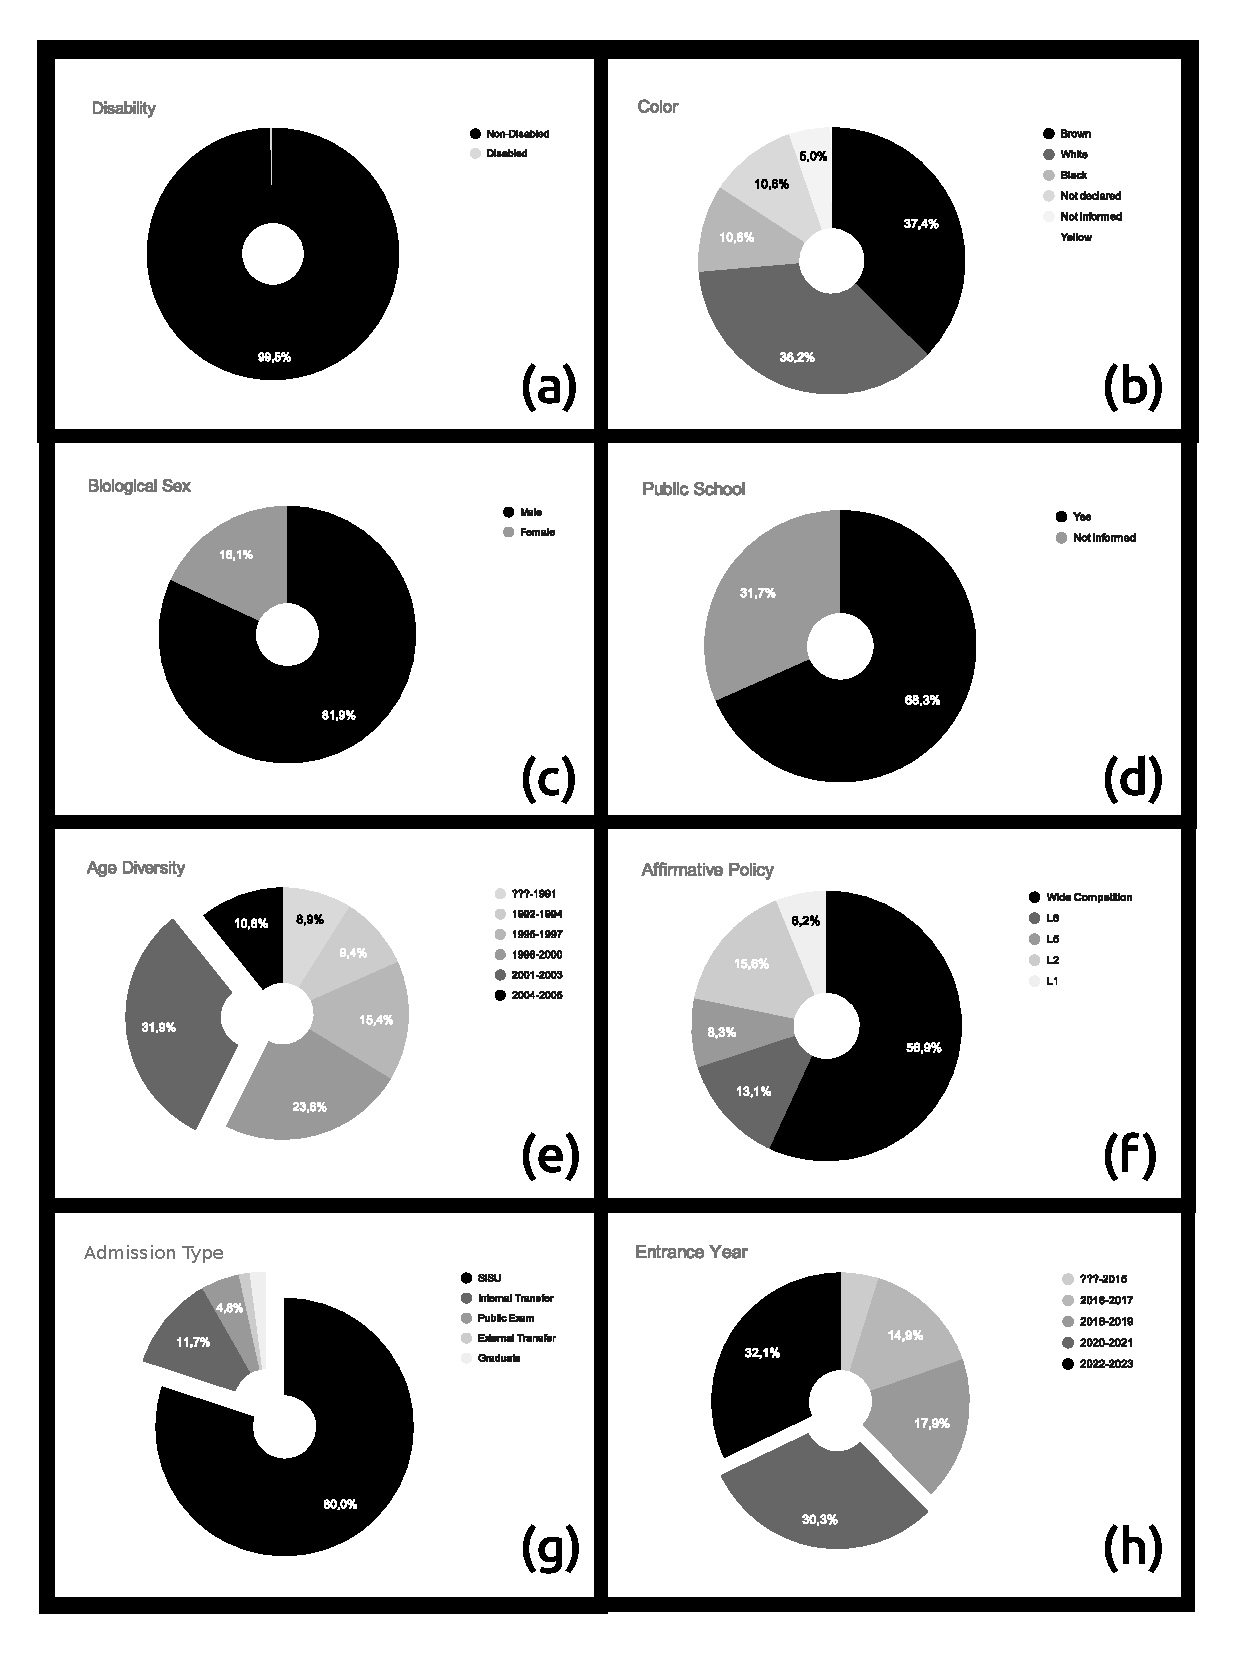
\includegraphics[width=0.9\textwidth]{images/chapter-08/all-charts-si-2023.pdf}}

\par\medskip\ABNTEXfontereduzida\selectfont\textbf{Source:} Created by the author (2024).
\end{figure}

% \fbox{
%     \begin{minipage}[htb]{0.9\textwidth}
%         \vspace{0.3cm}
                
%         \colorbox{gray!30}{% create a colored box
%             \makebox[0.975\textwidth][l]{% center the text on the page
%                 \ \ \textbf{Further Writing}
%             }
%         }

%         \vspace{0.1cm}
        
%         \begin{itemize}
%             \item Put here the aggregated report from UFPE Open Data:
%             \begin{itemize}
%                 \item situacao-academica-discentes-graduacao-2023-ufpe-atual.csv
%                 \item discentes-ingressos-sisu-2021-ufpe.csv
%                 \item discentes-ingressos-cursos-graduacao-2021-ufpe.csv
%                 \item beneficio-assistencia-estudantil-2023-proaes-ufpe.csv
%             \end{itemize}
%         \end{itemize}

%         \vspace{0.25cm}
        
%     \end{minipage}
% }

\subsection{Class Perspective}
\label{results-ss:classroom-data}

I divided the class perspective into three kinds of data sources: \gls{IS} program class planning, \acrfull{PBL} recordings, and socioeconomic form (see Table \ref{tbl:class-data-sources}).

\begin{table}[htb]
\caption{List of data sources from the class perspective (\acrshort{IS} program class planning, \acrshort{PBL} recordings, and socioeconomic form).}
\label{tbl:class-data-sources}
\centering
\rowcolors{1}{}{lightgray}
\begin{tabular}{
    >{\centering\arraybackslash}m{3cm}|
    >{\centering\arraybackslash}m{7cm}
}
    \hline
    \textbf{Abbreviation} &
    \textbf{Description} \\
    
    \hline
    \acrshort{DS-TP} &
    \acrshort{MIS} teaching plan \\
    
    \hline
    \acrshort{DS-PBL}1 &
    \acrshort{PBL}-Test data \\
    
    \acrshort{DS-PBL}2 &
    \acrshort{PBL-SEE} Output data \\

    \acrshort{DS-PBL}3 &
    \acrshort{PBL-SEE} Client Satisfaction data \\

    \acrshort{DS-PBL}4 &
    \acrshort{PBL-SEE} Performance data\\

    \acrshort{DS-PBL}5 &
    \acrshort{PBL-SEE} Content data\\

    \acrshort{DS-PBL}6 &
    \acrshort{PBL-SEE} Process data\\

    \hline
    \acrshort{DS-SEF} &
    Socioeconomic form data\\
    
    \hline
    
\end{tabular}

par\medskip\ABNTEXfontereduzida\selectfont\textbf{Source:} Created by the author (2024). \par\medskip

\end{table}

In \gls{IS} program class planning (\acrfull{DS-TP}), I collected \textbf{[DS-TP]} \gls{MIS} teaching plan 2023.1 (available in a sheet-structured format).

In \gls{PBL} recordings kind (\acrfull{DS-PBL}), I collected \textbf{[DS-PBL1]} \gls{PBL}-Test data and the assessment grades concerning each \gls{PBL-SEE} element: \textbf{[DS-PBL2]} output, \textbf{[DS-PBL3]} client satisfaction, \textbf{[DS-PBL4]} performance, \textbf{[DS-PBL5]} content, and \textbf{[DS-PBL6]} process. It is important to note that for each \gls{PBL-SEE} element, at least three data collection moments occurred through all \gls{PBL} cycles. I aggregated in Appendix \ref{chap:pbl-see-charts} all charts related to these \gls{PBL-SEE} elements. Generally, it is possible to assert that Chavo's and Quico's results in all assessment perspectives are similar, with Chavo's values slightly higher than Quico's in some situations but not disparate.

In the socioeconomic form kind (\acrfull{DS-SEF}), I collected \textbf{[DS-SEF]} a sort of data from the form available in Appendix \ref{chap:socio-quest}. I traced the Lorenz curve (Figure \ref{fig:lorenz-curve-classroom}) from each student's average household \textit{per capita} income in Chavo's and Quico’s class. I charted this curve with the data of 15 students who voluntarily answered the socioacademic questionnaire. Originally, this curve “plots the percentage of total income earned by various portions of the population when the population is ordered by the size of their incomes” \cite{gastwirth:1971}. But it helps compute several indexes to measure social inequalities, including under educational perspectives \cite{thomas:2003}. It assists us in visualizing the accumulated distribution of a certain quantity in a population.

\begin{figure}[ht!]
\centering

\caption{\textmd{Lorenz curve from average household \textit{per capita} income of Chavo and Quico’s class.}}
\label{fig:lorenz-curve-classroom}
\fcolorbox{gray}{white}{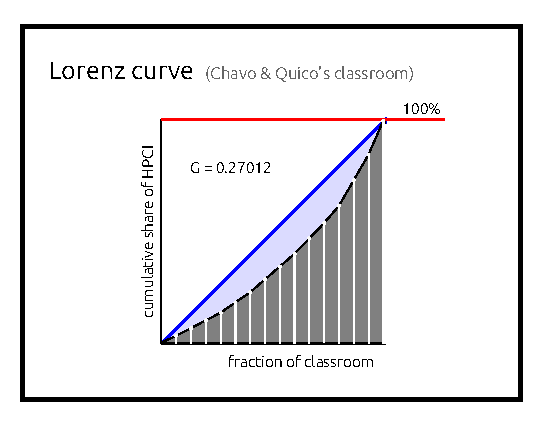
\includegraphics[width=0.9\textwidth]{images/chapter-08/lorenz-with-gini.pdf}}

\par\medskip\ABNTEXfontereduzida\selectfont\textbf{Source:} Created by the author (2024), assisted by Good Calculators (\url{http://goodcalculators.com}).%\citeauthor{manualufpe2020} (\citeyear{manualufpe2020}) \par\medskip
\end{figure}
%Data used for this chart creation :
%0.67,0.75,0.75,0.75,1.00,1.00,1.25,1.25,1.25,1.50,1.50,1.67,2.50,2.50,3.30

From Figure \ref{fig:lorenz-curve-classroom}, Chavo's and Quico's class (\acrfull{GI} $\approx$ 0.270) is closer to Finland (\gls{GI} = 0.277) than Brazil (\gls{GI} = 0.489)\footnote{Available in \url{https://data.worldbank.org/indicator/SI.POV.GINI?locations=BR}.} concerning incoming inequality. Indeed, as mentioned in Section \ref{res-meth-ss:lorenz}, \gls{GI} is a first indicator, and social inequality is a complex and multifactorial problem, but it can signal that even the Brazilian system of quotas (see Section \ref{equity-sec:br-context}) does not reflect significantly (in an \acrfull{CSE} class, for instance) the social inequality present in the Brazilian society.

Aiming to help me to choose strategically which two students I should investigate deeper (see Section \ref{res-met-ss:sampling-strategy}), I plotted the chart between student \acrfull{HPCI}s and the number of students in the \gls{MIS} class 2023.1 (Figure \ref{fig:sampling-classes-ds-sef}). I chose one \gls{CSE} undergraduate from \gls{Q}1 (Chavo) and another from \gls{Q}4 (Quico). Of all the students who volunteered themselves to participate in the interview moment, three belonged to \gls{Q}1, and two belonged to \gls{Q}4. I chose Chavo (\gls{HPCI} $\approx$ 0.67 Brazilian minimum wage) and Quico (\gls{HPCI} $\approx$ 2.50 Brazilian minimum wages), picking up one \gls{CSE} student in \gls{Q}1 and \gls{Q}4 respectively and at random.

\begin{figure}[ht!]
\centering

\caption{\textmd{Chart from average household \textit{per capita} income of Chavo and Quico’s class aiming to identify the four sampling classes (from \acrshort{Q}1 to \acrshort{Q}4).}}
\label{fig:sampling-classes-ds-sef}
\fcolorbox{gray}{white}{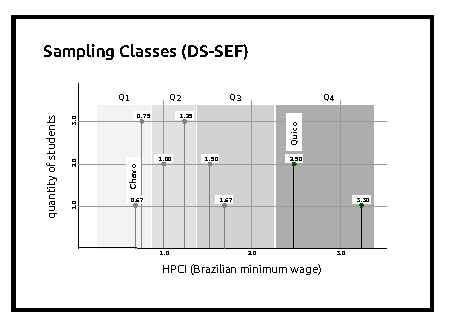
\includegraphics[width=0.9\textwidth]{images/chapter-08/collected-sampling-classes.pdf}}

\par\medskip\ABNTEXfontereduzida\selectfont\textbf{Source:} Created by the author (2024).%\citeauthor{manualufpe2020} (\citeyear{manualufpe2020}) \par\medskip
\end{figure}

% \vspace{0.3cm}

% \fbox{
%     \begin{minipage}[htb]{0.9\textwidth}
%         \vspace{0.3cm}
                
%         \colorbox{gray!30}{% create a colored box
%             \makebox[0.975\textwidth][l]{% center the text on the page
%                 \ \ \textbf{Further Writing}
%             }
%         }

%         \vspace{0.1cm}
        
%         \begin{itemize}
%             \item Creating a table with all data concerning the grades of MIS students.
%         \end{itemize}

%         \vspace{0.25cm}
        
%     \end{minipage}
% }

% \vspace{0.3cm}




